\documentclass[a4paper,11pt]{exam}
%\printanswers % pour imprimer les réponses (corrigé)
 %\noprintanswers % Pour ne pas imprimer les réponses (nonc)
% \addpoints % Pour compter les points
% \noaddpoints % pour ne pas compter les points
\qformat{\textbf{Exercice \thequestion \,:}\\} % Questions style
\usepackage{color} % Define new colors

\usepackage[utf8x]{inputenc}
\usepackage[T1]{fontenc}
\usepackage{exercise}
\usepackage{mathrsfs,amsmath,amssymb,latexsym,amsfonts,mathtools,stmaryrd}
\usepackage{enumitem}
\setitemize{label=\textbullet}
% Bigger binomial in math mode
\usepackage{nccmath}
\renewcommand{\binom}{\mbinom}

\usepackage[francais]{babel}

\shadedsolutions % définit le style des réponses
% \framedsolutions % définit le style des réponses 
\definecolor{SolutionColor}{rgb}{0.8,0.9,1} % bleu ciel
\renewcommand{\solutiontitle}{
\noindent\textbf{Solution:}\par\noindent} % Définit le titre des réponses
\newcommand\eqdef[0]{\stackrel{\text{def}}{=}}

\pagestyle{headandfoot}
\headrule
\header{L3 - 2019/2020 - TD2}{Mercredi 25 septembre}{Mathématiques discrètes}
\footer{S. Le Roux, I. Khmelnitsky}{\thepage}{E.N.S. Cachan}
\footrule

\renewcommand{\questionshook}{%
  \setlength{\labelwidth}{0pt}%
  \setlength{\itemsep}{0.9\baselineskip}
}

\definecolor{gris}{gray}{0.95}
\newcommand{\Z}{\mathbb{Z}}
\newcommand{\N}{\mathbb{N}}
\newcommand{\Q}{\mathbb{Q}}
\newcommand{\R}{\mathbb{R}}
\newcommand{\C}{\mathbb{C}}
\newcommand{\F}{\mathbb{F}}
\newcommand{\res}{\mathcal{R}}

\begin{document}

\begin{center}

\underline{Leftovers from last week:}
\end{center}

~\vspace{-0.6cm}
\begin{enumerate}
	\item Show that $\forall (n_r,n_b)\in\mathbb{N}^2, \exists N\in\mathbb{N}$
	such that, for any $2$ (edge) coloring $\{r,b\}$ of the complete graph
	$K_N$, there exists a color $c\in\{r,b\}$ for which there is a complete sub-graph $K_{n_c}$ which is monochromatic in the color $c$.
	\\
	(the smallest $N$ for which this property holds is denoted by $R(n_r,n_b)$).
	
	\begin{solution}
		We show this by induction on $n_r + n_b$. First note that $R(n,1) = R(1,n)=1$.
		To show that $R(n_r,n_b)$ exists we'll show that $R(n_r, n_b) \leq R(n_r-1, n_b) + R(n_r, n_b-1)$. 
		
		Consider the complete graph on $ R(n_r-1, n_b) + R(n_r, n_b-1) $ edges. Pick a vertex $v$. Partition the rest of the edges in to 2 sets $R$ and $B$, where for any $u\in R$ the edge $(u,v)$ is colored red and for any $u\in B$ the edge $(u,v)$ is colored blue. Now, since $ R(n_r-1, n_b) + R(n_r, n_b-1) = 1 + |R|+|B|$ either $|R|>R(n_r-1, n_b)$ or $|B|>R(n_r, n_b-1)$. First assume that $|R|>R(n_r-1, n_b)$. The sub-graph induced on the vertices of $ R $ either has a complete monochromatic blue sub-graph on $ n_b $ vertices and we are done, or it has a complete monochromatic red sub-graph on $ n_r-1 $ vertices and adding the vertex $v$ produces a complete monochromatic red sub-graph on $ n_r $ vertices and we are done. If $|B|>R(n_r, n_b-1)$, the same proof works by reversing the colors.
	\end{solution}
	
	\item Show that $\forall k\in\mathbb{N},\forall (n_1, n_2, \dots,
	n_k)\in\mathbb{N}^k, \exists N\in\mathbb{N}$ such that, for any $k$ (edge) coloring of the complete graph $K_N$, there exists a color $c\in\llbracket 1,k \rrbracket$ for which there is a complete sub-graph $K_{n_c}$ which is monochromatic in the color $c$.
	\\ (the smallest $N$ for which this property holds is denoted by $R(n_1,\dots,n_k)$).
	
	\begin{solution}
		By induction on $k$ We'll show that $R(n_1,\dots,n_k)\leq R(n_1,\dots,n_{k-2},R(n_{k-1},n_k)) $. For $k=2$ we've shown it in the previous exercise.
		Let $k>2$ and take a graph of size $ R(n_1,\dots,n_{k-2},R(n_{k-1},n_k))$. Now, imagine that we became partially color blind and stop differentiating between the colors $n_{k-1}$ and $n_k$ and instead see a new color. By induction our graph either admits a complete monocromatic sub-graph in the color $c$ of size $n_c$ for $c\in [n-2]$ and we are done, or it admits a complete monocromatic sub-graph $ G $ in the new color of size $R(n_{k-1},n_k)$. Now, imagine our eyes can suddenly see the difference between the $n_{k-1},n_k$. We get a 2 colored graph of size $R(n_{k-1},n_k)$ and from what we have shown in the previous exercise we are done.
	\end{solution}
\end{enumerate}
\bigskip
\bigskip
\begin{questions}

  \setcounter{question}{-1}
  \question % Preuves non faites en cours
  ~\vspace{-0.5cm}
  \begin{enumerate}
    \item Let $E$ and $F$ two countable sets. 
      Show that $E \cup F$ is countable.

      \begin{solution}
      	Let $f$ (resp.\ $g$) be 1-1 functions from $E$ (resp.\ $F$) to $\N$. We construct a new function:
      	\[
      	\begin{array}{rl}
      	E \cup F & \mapsto \N \\
      	x & \rightarrow \left\{
      	\begin{array}{ll}
      	2f(x) & \text{si } x \in E \\
      	2g(x)+1 & \text{si } x \in F \setminus E
      	\end{array}
      	\right.
      	\end{array}
      	\]
      	It is also 1-1 and hence $E \cup F$ is countable.
      \end{solution}

    \item Let $E_1, \dots, E_n$ be countable sets. 
      Show that $\prod_{i=1}^n E_i$ is countable.

      \begin{solution}
      	Denote by $f_i$ a 1-1 function from $E_i$ to $\N$. We construct a new function:
       
        \[
          \begin{array}{rl}
          \prod_{i=1}^n E_i & \mapsto \N^n \\
          x & \rightarrow (f_i(x))_{1 \leq i \leq n}
          \end{array}
        \]
        Since $\N^n$ is countable, so is $\prod_{i=1}^n E_i$.
      \end{solution}
  \end{enumerate}

  \vspace{0.6cm}
  \colorbox{gris}{
    \begin{minipage}[c]{\textwidth}
      Combinatorial reasoning
    \end{minipage}
  }~
  \vspace{-0.1cm}

  \question
  Demonstrate by combinatorial arguments the identity:
  \[
    \forall n\in\N,~\binom{3n}{3} = 3\binom{n}{3} + 6n\binom{n}{2} + n^3
  \]

  \begin{solution}
  	Partition the set of size $3n$ to 3 partitions of the same size, and color the in 3 different colors.
  	To Pick 3 elements form this set we can either pick 3 elements of the same color($3\binom{3n}{3}$), pick two with the same color and the third one in a different color($ 6n\binom{n}{2} $) and pick 3 of different color($n^3$). Summing up we get:
  	 \[
  		\binom{3n}{3} = 3\binom{n}{3} + 6n\binom{n}{2} + n^3
  	\]
  \end{solution}

  \vspace{0.6cm}
\colorbox{gris}{
	\begin{minipage}[c]{\textwidth}
		Applications of the pigeonhole principle 
	\end{minipage}
}~
\vspace{-0.1cm}

  \question
  Some arcs of a circle with a diameter $1$ were colored. The sum of the lengths of the colored arcs is $>\pi/2$.
  Show that there exists a diameter of the circle, for which both ends are colored.

  \begin{solution}
  	Assume for contradiction that there doesn't exists a diameter with both edges colored.
  	This means that for every colored arch there is a symmetrical arch which is not colored. Therefore the sum of the lengths of the none colored arches is also $>\pi/2$, but we know that the length of the circumference is $\pi*d = \pi$ which gives us a contradiction ot our assumption.

  \end{solution}


  \question
  Let $m_1,...,m_{n+1}$ be $n+1$ numbers, chosen from the set $[2n]$.\\
  Show that there exist a pair $i,j$, $1 \leq i \neq j \leq n+1$ such that $m_i$ is divisible by
  $m_j$.

  \begin{solution}
  	Each of the chosen numbers can be represented as $2^{k_i} q_i$ where $k_i\in\N$ and $q_i$ is one of the $n$ odd numbers in $[2n]$. From the pigeonhole principle there are at least two chosen numbers $m_i,m_j$ for which $q_i=q_j$ and $k_i<k_j$. Therefore $m_j \mod m_i = 0$.
  \end{solution}

  \vspace{0.8cm}
  \colorbox{gris}{
    \begin{minipage}[c]{\textwidth}
       Cardinalities. 
    \end{minipage}
  }~
  \vspace{-0.1cm}

  \question
  Show that the family of all the finite sets of $\N$ is countable.

  \begin{solution}
  	1. The family of finite  sets of $\N$ is equal to $ \cup_{n\in\N }\mathcal{P}([n])	$, which is a countable union of finite sets.
  	
  	2. Build a 1-1 function from family of all the finite sets of $\N$: 
  	\[
  		f(A) = \sum_{k\in A} 2^k
  	\] 
   	$ f(A)\in \N$ since $A$  is finite, and for $ A\neq B $ we have $f(A)\neq f(B)$.
  \end{solution}

  \question
  Show that the set of decimal numbers is countable.

  \begin{solution}
  	Every decimal number can be represented as 3 natural numbers, before the decimal point, the number of zeros after the decimal point and before the first non zero number, and the number after the last zero.

  \end{solution}

  \question
  Let $\Sigma$ be a finite alphabet.
  % Soit $\Sigma^*$ l'ensemble des mots finis sur l'alphabet $\Sigma$.
  \begin{enumerate}
    \item Show that the set of finite trees on $\Sigma$ is countable.
   

      \begin{solution}
        This is a countable of union of finite sets, where we partition according to the size of the tree.
      \end{solution}

    \item Show that $\Sigma^\infty$ isn't countable (unless it $|\Sigma| = 1$)

      \begin{solution}
      	Diagonal argument: Assume for contradiction that it is countable, hence there is a onto function $f:\N\mapsto \Sigma^\infty$. Pick two different letters $a,b\in\Sigma$. 
      	Let $w$ be the word where:
      	\[
      		\forall n\in\N;w_{n}=\begin{cases}
      		a & f(n)_{n}\neq a\\
      		b & \text{otherwise}
      		\end{cases}
      	\] 
      	The word $w$ doesn't  $n\in\N$ for which $f(n) = w$, which gives us the contradiction. 
      \end{solution}
  \end{enumerate}

 
  \question
  Give an example of an uncountable family $F\subseteq P(\N)$, such that for any $A\neq B\in F$, $A\cap B$ is finite.

  \begin{solution}
    We saw in previous exercise that the family of infinite sequences of $\{0,1\}$ is uncountable. For each sequence $\{a_n\}_{n\in\N}$ in this family let: 
    \[ 
    	U_a:=\left\{\sum_{i=1}^n2^{a_i} \mid n\in\N\right\}
    \]    
    This is an uncountable family. For any two sequences $\{a_n\}_{n\in\N}$ and $\{b_n\}_{n\in\N}$ the intersection of $U_a\cap U_b$ is finite, since $\exists m\in \N$ s.t. $a_m \neq b_m$ and therefore for any $k\geq m$:
	\[ 
	  \sum_{i=1}^k2^{a_i} \neq \sum_{i=1}^k2^{b_i}.
	\] 
  \end{solution}
	

  \question
  By using Cantor–Schröder–Bernstein theorem, show that $\{0,1\}^\N$, $\N^\N$ and $\R$
  are equipotent.

  \begin{solution}
%  	We need to find to 1-1 functions. For the function from $\N^\N$ to $\R$ we can take for any
%    $(u_i)_{i\in\N}$ the real number:
%    \[
%      0.
%      0 \underbrace{1 \cdots 1}_{u_0}
%      0 \underbrace{1 \cdots 1}_{u_1}
%      0 \underbrace{1 \cdots 1}_{u_2}
%      0 \cdots
%    \]
    For the function from $\R$ to $\N^\N$, any $ x\in\R $ can be represented in the following way $sg(x)(\lfloor |x| \rfloor, x_1 x_2 x_3 \cdots)$, and we map it to:
    \[
      (sg(x)+1, \lfloor |x| \rfloor. x_1 x_2 x_3 \ldots)
    \]
    For the the function from $\{0,1\}^\N$ to $\R$, for any $ (x_n)_{n=1}^\infty \in \{0,1\}^\N$  we get:
    \[
    	0.x_1 x_2 x_3 \cdots
    \]
    For the the function from $\N^\N$ to $\{0,1\}^\N$, for any $ (y_n)_{n=1}^\infty \in \N^\N$  we get:
        \[
          0 \underbrace{1 \cdots 1}_{y_1}
          0 \underbrace{1 \cdots 1}_{y_2}
          0 \underbrace{1 \cdots 1}_{y_3}
          0 \cdots
        \]
  \end{solution}
  \qformat{\textbf{Exercice \thequestion \,:}\\}
 \question Another way to show that $[0,1]$ is a uncountable set.\\
 Let $\{x_n\}_{n\in \N}$ a series of real numbers in the interval $[0,1]$.
 \begin{enumerate}
 	\item Construct recursively a sequence of closed intervals $I_n$ of length $>0$ such that~:
 	\begin{itemize}
 		\item $I_0 \subset [0,1]$, 
 		\item $I_n \subset I_{n-1}$,
 		\item $I_n$ are intervals of length $>0$ that do not contain $x_n$.
 	\end{itemize}
 	
 	\begin{solution}
 		Let construct the sequence recursively(this is one of the options to do it)~:
 		\begin{itemize}
 			\item $I_{0} = [0,1]$.
 			\item  For $n \geq 0$ with $I_{n-1} = [a_{n-1}, b_{n-1}]$,
 			\[
 			I_n = \left\{
 			\begin{array}{ll}
 			I_{n-1} & \text{si } x_n \notin I_{n-1} \\
 			{}[\frac{x_n+b_{n-1}}{2},b_{n-1}] & \text{si } x_n \in
 			[a_{n-1}, b_{n-1}[ \\
 			{}[a_{n-1},\frac{a_{n-1}+b_{n-1}}{2}] & \text{si }
 			x_n=b_{n-1}
 			\end{array}
 			\right.
 			\]
 		\end{itemize}
 	\end{solution}
 	
 	\item Deduce that $ [0,1] $ is uncountable.
 	
 	\begin{solution}
 		In the first part we constructed a sequence of nested closed non-empty intervals, by Cantor's intersection theorem we can deduce that $\cap_n I_n\neq \emptyset$. Moreover, for any $n\in\N$ $x_n\notin \cap_n I_n$. Therefore we can conclude that for any countable sequance of real  numbers in $[0,1]$ there is always $y\in[0,1]$ for which there is no $n\in\N$ for which $x_n = y$.
 	\end{solution}
 \end{enumerate}

\qformat{\textbf{Exercise \thequestion~(\thequestiontitle):}\\}
\titledquestion{Stern–Brocot tree}
In this exercise we'll show a way to represent strictly positive rational numbers in the form of an infinite binary tree.

We start we two imaginary vertices $0/1$ (which represents $0$) and $1/0$ (which represent infinity).
Each step we insert between each two of the consecutive fractions $m_1/n_1$ and $m_2/n_2$ the fraction ${(m_1+m_2)/(n_1+n_2)}$.

Thus, we obtain after four stages:


\begin{minipage}{0.4\textwidth}
	\begin{enumerate}[label=\arabic*)]
		\item init : $[\frac{0}{1}, \frac{1}{0}]$
		\item $[\frac{0}{1}, \frac{1}{1}, \frac{1}{0}]$
		\item $[\frac{0}{1}, \frac{1}{2}, \frac{1}{1}, \frac{2}{1}, \frac{1}{0}]$
		\item $[\frac{0}{1}, \frac{1}{3}, \frac{1}{2}, \frac{2}{3},
		\frac{1}{1}, \frac{3}{2}, \frac{2}{1}, \frac{3}{1}, \frac{1}{0}]$
		\item $[\frac{0}{1}, \frac{1}{4}, \frac{1}{3}, \frac{2}{5},
		\frac{1}{2}, \frac{3}{5}, \frac{2}{3}, \frac{3}{4}, \frac{1}{1},
		\frac{4}{3}, \frac{3}{2}, \frac{5}{3}, \frac{2}{1}, \frac{5}{2},\\
		\frac{3}{1}, \frac{4}{1}, \frac{1}{0}]$
	\end{enumerate}
\end{minipage}
\begin{minipage}{0.5\textwidth}
	\begin{center}
		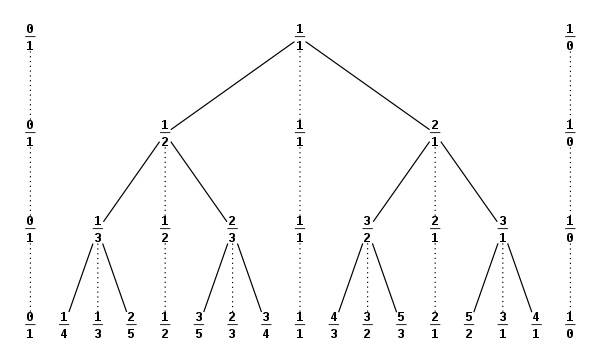
\includegraphics[scale=0.5]{alg_val_han.png}
	\end{center}
\end{minipage}

\begin{enumerate}
	\item Verify that for $m_1/n_1 < m_2/n_2$, we have $m_1/n_1 < (m_1+m_2)/(n_1+n_2) < m_2/n_2$.
	
	\begin{solution}
		\[
		\frac{m_1+m_2}{n_1+n_2}-\frac{m_1}{n_1} = \frac{m_2n_1-m_1n_2}{n_1(n_1+n_2)} =
		\frac{n_2(m_2/n_2-m_1/n_1)}{n_1+n_2} > 0
		\]
		and a similar equation on the other side.
		\[
		\frac{m_1+m_2}{n_1+n_2}-\frac{m_2}{n_2} = \frac{m_1n_2-m_2n_1}{n_1(n_1+n_2)} =
		\frac{n_2(m_1/n_1-m_2/n_2)}{n_1+n_2} < 0
		\]
		
	\end{solution}
	
	\item  Show that for any step and for any two consecutive fractions $m_1/n_1 < m_2/n_2$, we have $n_2m_1 - m_2n_1 = \pm 1$.
	
	\begin{solution}
		We show this inductively: For the first step this is correct.
		$n_1(m_1+m_2)-(n_1+n_2)m_1 = (n_1m_2-m_1n_2)$ and $n_2(m_1+m_2)-(n_1+n_2)m_2= (n_2m_1-m_2n_1)$.
	\end{solution}
	
	\item Deduce that the fractions constructed by this process are in an irreducible form (i.e. the numerator and the denominator greatest common divisor is 1).
	
	\begin{solution}
		Assume for contradiction that there exists a $d\neq 1$ which divides both $m_1$ and $n_1$. From previous exercise  we know that $n_2m_1 - m_2n_1 = \pm1$.  But then dividing both sides of the equation by $d$ we get on one side a whole number but on the other a fraction, which gives us a contradiction to our assumption.
	\end{solution}
	
	\item Let $p/q$ be a strictly positive rational represented by an irreducible fraction. Suppose that $\frac{m_1}{n_1} < \frac{p}{q} <
	\frac{m_2}{n_2}$ and show that $m_1+m_2+n+n_2 \leq p+q$ (where $\frac{m_1}{n_1}$ and $\frac{m_2}{n_2}$ are two consecutive fractions ).
	
	\begin{solution}
		We have : $pn_1-qm_1 \geq 1$(they are whole numbers $pn_1-qm_1>0$) and $m_2q-n_2p \geq 1$. Therefore:
		\begin{align*}
		m_1+m_2+n_1+n_2 & \leq (m_1+n_1)(m_2q-n_2p)+(m_2+n_2)(pn_1-qm_1) \\
		& = p(n_1(m_2+n_2)-n_2(m_1+n_1))+q(m_2(m_1+n_1)-m_1(m_2+n_2)) \\
		& = p\underbrace{(n_1m_2-m_1n_2)}_1+q\underbrace{(n_1m_2-m_1n_2)}_1 \\
		& = p+q
		\end{align*}
	\end{solution}
	
	\item Let $p/q$ be a strictly positive rational number represented by an irreducible fraction. Show that it appears uniquely in the construction.
	
	\begin{solution}
		We make induction on $p+q$.
		
		For $p+q=2$, $p=1$ and $q=1$ and $1/1$ appeared in the first step.
		
		Au début, $\frac{0}{1} < \frac{p}{q} < \frac{1}{0}$.
		On raffine petit à petit cet encadrement.
		
		If $\frac{m_1}{n_1} < \frac{p}{q} < \frac{m_2}{n_2}$, then there are 3 possibilities~:
		\begin{itemize}
			\item $\frac{m_1+m_2}{n_1+n_2} = \frac{p}{q}$.	
			\item $\frac{m_1}{n_1} < \frac{p}{q} < \frac{m_1+m_2}{n_1+n_2}$, but then 
			$m_1+m_2+n_1+n_2 < m_1+m_1+m_2+n_1+n_1+n_2 \leq p+q$.
			\item $\frac{m_1+m_2}{n_1+n_2} < \frac{p}{q} < \frac{m_2}{n_2}$, but then  
			$m_1+m_2+n_1+n_2 < m_1+m_2+m_2+n_1+n_2+n_2 \leq p+q$.
			
		\end{itemize}
		
		Therefore since the sum $m_1+m_2+n_1+n_2$ strictly increasing on each level, we get that after at most $p+q$ levels we'll find $p/q$ 
	\end{solution}
	
	\item Conclude that $\Q^{*+}$ is countable. 
	
	\begin{solution}
		We get that $\Q^{*+}$ is a union of $\N$ finite sets.
	\end{solution}
\end{enumerate}

 
%  
%  \qformat{\textbf{Exercice \thequestion~(\thequestiontitle):}\\}
%  \titledquestion{Cantor's set}
%  Let $ I= [a,b]$ an interval of length $\delta = b-a$.
%  Let $ \rho(I) =[a, a + \frac {\delta} {3}] \cup [b- \frac{\delta}{3}, b] $. $\rho$ cuts the interval $ I $ in to three closed intervals of equal length and removes the middle one. 
%  We extend $\rho$ to closed unions of disjointed closed intervals by making $\rho$ act on each of the intervals separately.
%  
%
%  Cantor set is $ C = \cap_n F_n $, where $F_n$ is defined recursively on $n$:
%  \[
%    F_0 = [0,1] \textrm{ and } F_n = \rho(F_{n-1})
%  \]
%
%  \begin{enumerate}
%    \item Show that $C$ is closed, non-empty and of "length" 0(We mean the length of the sum of the intervals contained in it (but what we really want to say is the measure :) )).
%      
%      \begin{solution}
%      	By construction each $F_n$ is closed and subset of $F_{n-1}$. By Cantor's intersection theorem we get that $C = \cap_n F_n$ is non-empty and closed. Moreover, we have that for any $n$, $\mu(F_n)=\frac{2}{3}\mu(F_{n-1})$. Therefore for any $n$, $\mu(C)\leq (\frac{2}{3})^n$, and by taking the limit we get that $\mu(C) = 0$.
%
%      \end{solution}
%
%    \item 
%     Let $n \in \N$. Show that $F_n$ is a union of $2^n$
%    intervals $\cup_{i=1}^{2^n} [a_i,b_i]$. The ordered sequence
%    $a_0, a_1,\dots,a_{2^n}$ where the items are of the form $\frac{\sum_{i=1}^{n} x_i3^i}{3^n}$, where $x_i \in \{0,2\}$
%    (elements of $[0,1]$ in base $3$ which have at most $n$
%    digits and constitute of $0$ and $2$) and
%    $b_i = a_i + \frac{1}{3^n}$.
%%    
%%    Soit $n \in \N$. Démontrer que $F_n$ est la réunion de $2^n$
%%      intervalles $\cup_{i=1}^{2^n} [a_i,b_i]$, la suite
%%      $a_0, a_1,\dots,a_{2^n}$ représente la suite ordonnée des éléments de la
%%      forme $\frac{\sum_{i=1}^{n} x_i3^i}{3^n}$, avec $x_i \in \{0,2\}$
%%      (éléments de $[0,1]$ dont le développement en base $3$ a au plus $n$
%%      chiffres et ne comporte que des $0$ et des $2$) et
%%      $b_i = a_i + \frac{1}{3^n}$.
%
%      \begin{solution}
%        We show this by induction on $n$.
%
%        This is true for $F_0=[0,1]$ where $a_0=0$ and
%        $b_0=1=a_0+\frac{1}{3^0}$. \\
%        Assume that $F_n=\sqcup_{i=1}^{2^n} [a_i,b_i]$ with $a_0, a_1, \dots,
%        a_{2^n}$ ordered sequence of the form
%        $\frac{\sum_{j=1}^{n} x_j3^j}{3^n}$ and $b_i = a_i + \frac{1}{3^n}$,
%        for all $i$.
%        
%        Let $F_{n+1} = \rho(F_n) = \sqcup_{i=1}^{2^n} \rho([a_i,b_i])$.
%        By definition, $\rho([a_i,b_i]) = [a_i,a_i+\frac{1}{3^{n+1}}] \cup
%        [b_i-\frac{1}{3^{n+1}},b_i]$.
%
%        Let $c_{2i}=a_i$, $d_{2i}=a_i+\frac{1}{3^{n+1}}$,
%        $c_{2i+1}=b_i-\frac{1}{3^{n+1}}$, $d_{2i+1}=b_i$, where
%        \[
%        F_{n+1}=\cup_{i\in[n]}\left([c_{2i},d_{2i}] \cup [c_{2i+1},d_{2i+1}]\right)
%        \] with
%        $c_{2i}<d_{2i}<c_{2i+1}<d_{2i+1}$.
%
%        Doing some computation we get~:
%        \begin{itemize}
%          \item $c_{2i} = a_i = \frac{\sum_{j=1}^{n} x_j3^j}{3^n} =
%            \frac{\sum_{j=1}^{n} x_j3^{j+1}}{3^{n+1}}$,
%          \item $d_{2i} = a_i + \frac{1}{3^{n+1}} = c_{2i} +
%            \frac{1}{3^{n+1}}$,
%          \item $c_{2i+1} = b_i - \frac{1}{3^{n+1}} =
%            a_i +\frac{1}{3^n} - \frac{1}{3^{n+1}} = 
%            c_{2i} + \frac{2}{3^{n+1}} = 
%            \frac{2+\sum_{j=1}^{n} x_j3^{j+1}}{3^{n+1}}$,
%          \item $d_{2i+1} = b_i = c_{2i+1} + \frac{1}{3^{n+1}}$. 
%        \end{itemize}
%      \end{solution}
%
%    \item Deduce that $C$ consists of all the numbers in $[0,1]$ whose base $3$ representation has only $0$'s and $2$'s.
%
%      \begin{solution}
%      	Les éléments de l'intervalle $[a_i,b_i]$ avec
%      	$a_i=\frac{\sum_{j=1}^n x_j 3^j}{3^n}$ et
%      	$b_i=a_i+\frac{1}{3^n}$ sont exactement les éléments dont le
%      	développement triadique $\sum_{j=1}^{\infty}\frac{y_j}{3^j}$ vérifie
%      	$y_1 = x_1, \dots, y_n = x_n$.
%      	
%        Les éléments de l'intervalle $[a_i,b_i]$ avec
%        $a_i=\frac{\sum_{j=1}^n x_j 3^j}{3^n}$ et
%        $b_i=a_i+\frac{1}{3^n}$ sont exactement les éléments dont le
%        développement triadique $\sum_{j=1}^{\infty}\frac{y_j}{3^j}$ vérifie
%        $y_1 = x_1, \dots, y_n = x_n$.
%      \end{solution}
%
%    \item Build a bijection from $C$ to $[0,1]$, using the previous exercise.
%
%      \begin{solution}
%        The bijection is~:
%        \begin{align*}
%          C & \mapsto [0,1] \\
%          \sum_{j=1}^{\infty}\frac{y_j}{3^j} & \rightarrow
%          \sum_{j=1}^{\infty}\frac{y_j/2}{2^j}
%        \end{align*}
%
%      \end{solution}
%
%    \item Deduce that $C$ is uncountable.
%
%      \begin{solution}
%       There is a bijection from $C$ to $[0,1]$.
%      \end{solution}
%  \end{enumerate}
\end{questions}

\end{document}
% vim: spell spelllang=fr
